\documentclass[12pt,letterpaper]{article}
\usepackage[utf8]{inputenc}
\usepackage[spanish]{babel}
\usepackage{graphicx}
\usepackage[left=2cm,right=2cm,top=2cm,bottom=2cm]{geometry}
\usepackage{graphicx} % figuras
% \usepackage{subfigure} % subfiguras
\usepackage{float} % para usar [H]
\usepackage{amsmath}
%\usepackage{txfonts}
\usepackage{stackrel} 
\usepackage{multirow}
\usepackage{enumerate} % enumerados
\renewcommand{\labelitemi}{$-$}
\renewcommand{\labelitemii}{$\cdot$}
% \author{}
% \title{Caratula}
\begin{document}

% Fancy Header and Footer
% \usepackage{fancyhdr}
% \pagestyle{fancy}
% \cfoot{}
% \rfoot{\thepage}
%

% \usepackage[hidelinks]{hyperref} % CREA HYPERVINCULOS EN INDICE

% \author{}
\title{Caratula}

\begin{titlepage}
\begin{center}
\large{UNIVERSIDAD PRIVADA DE TACNA}\\
\vspace*{-0.025in}
\begin{figure}[htb]
\begin{center}

\includegraphics[width=8cm]{./Imagenes/logo}
\end{center}
\end{figure}
\vspace*{0.15in}
INGENIERIA DE SISTEMAS  \\

\vspace*{0.5in}
\begin{large}
TITULO:\\
\end{large}

\vspace*{0.1in}
\begin{Large}
\textbf{INFORME DE LABORATORIO 03} \\
\end{Large}

\vspace*{0.3in}
\begin{Large}
\textbf{CURSO:} \\
\end{Large}

\vspace*{0.1in}
\begin{large}
INTELIGENCIA DE NEGOCIOS\\
\end{large}

\vspace*{0.3in}
\begin{Large}
\textbf{DOCENTE:} \\
\end{Large}

\vspace*{0.1in}
\begin{large}
 Patrick Cuadros Quiroga\\
\end{large}

\vspace*{0.2in}
\vspace*{0.1in}
\begin{large}
Integrantes: \\
\begin{flushleft}


Mamani Ayala, Brandon     \hfill	(2015052715) \\

\end{flushleft}
\end{large}
\end{center}

\end{titlepage}


\tableofcontents % INDICE
\thispagestyle{empty} % INDICE SIN NUMERO
\newpage
\setcounter{page}{1} % REINICIAR CONTADOR DE PAGINAS DESPUES DEL INDICE

\section{Desarrollo } 


 EJERCICIO 1

\begin{itemize}
\item Tarea 1 : Conectar a datos existentes


\begin{enumerate}
\item Abrir SQL Server Management Studio y conectar a la intancia de base de datos (local) utilizando autenticacion de Windows 

\begin{center}
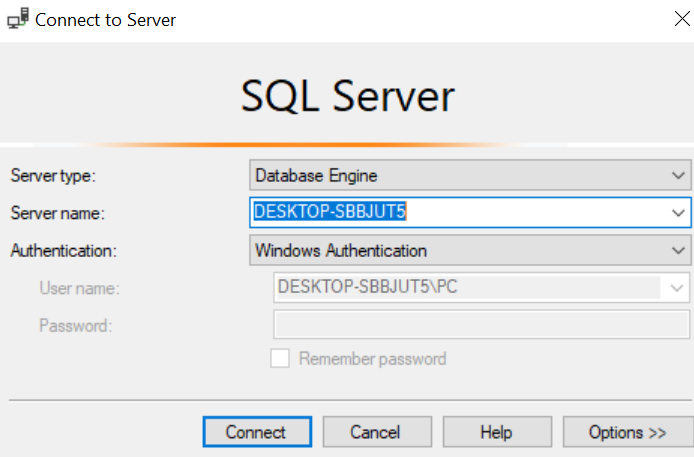
\includegraphics[scale=0.55]{./Imagenes/1.png}
\end{center}

\item Abrir la solucion Project.ssmssln , cuando carge expandir las Conultas (Queries) y hacer click en Exercise1.sql

\begin{center}
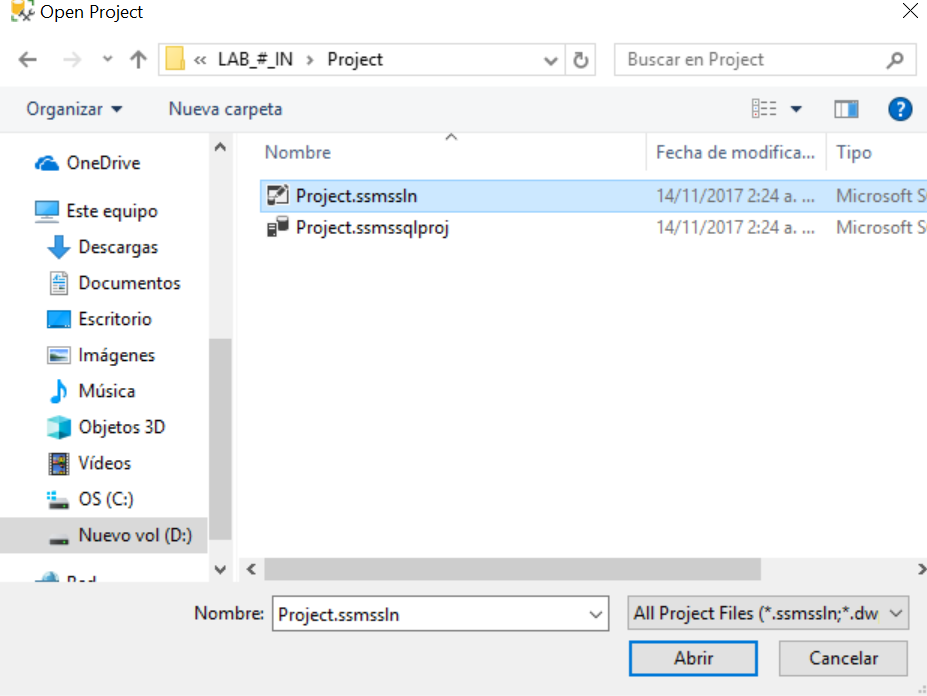
\includegraphics[scale=0.55]{./Imagenes/2.png}
\end{center}

\begin{center}
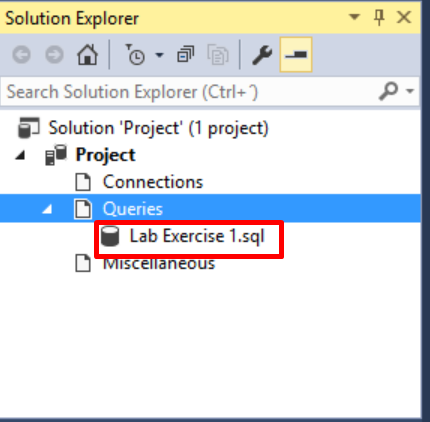
\includegraphics[scale=0.55]{./Imagenes/3.png}
\end{center}

\item Abrir PowerBI Desktop y conectar con la base de datos AdventureWorksLT2016 . Seguidamente expandir las opciones avanzadas y copiar el Task 1 del Lab Exercise 1.sql en la descripcion. 

\begin{center}
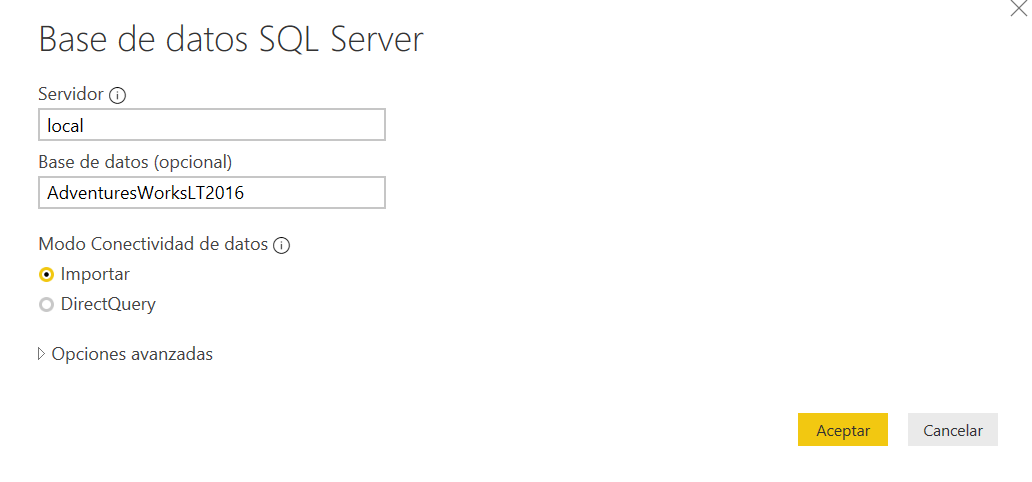
\includegraphics[scale=0.55]{./Imagenes/6.png}
\end{center}

\begin{center}
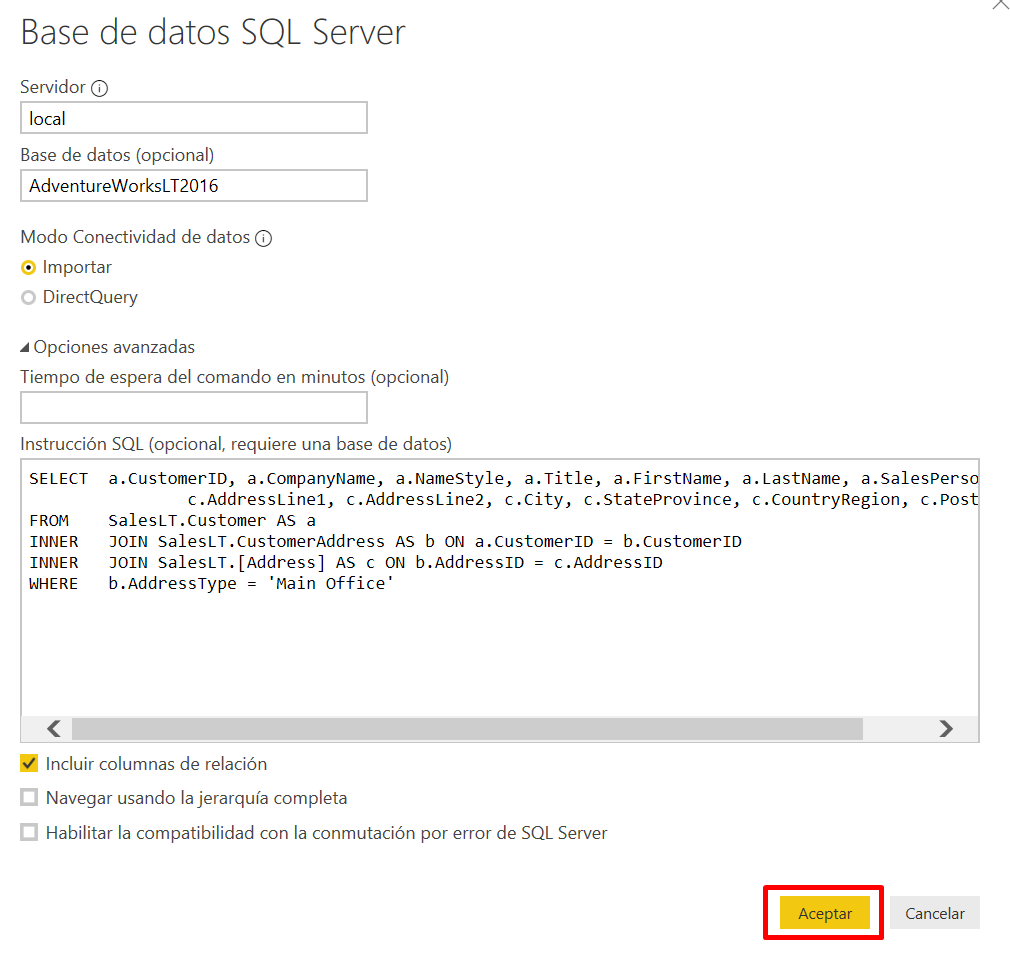
\includegraphics[scale=0.55]{./Imagenes/7.png}
\end{center}

\begin{center}
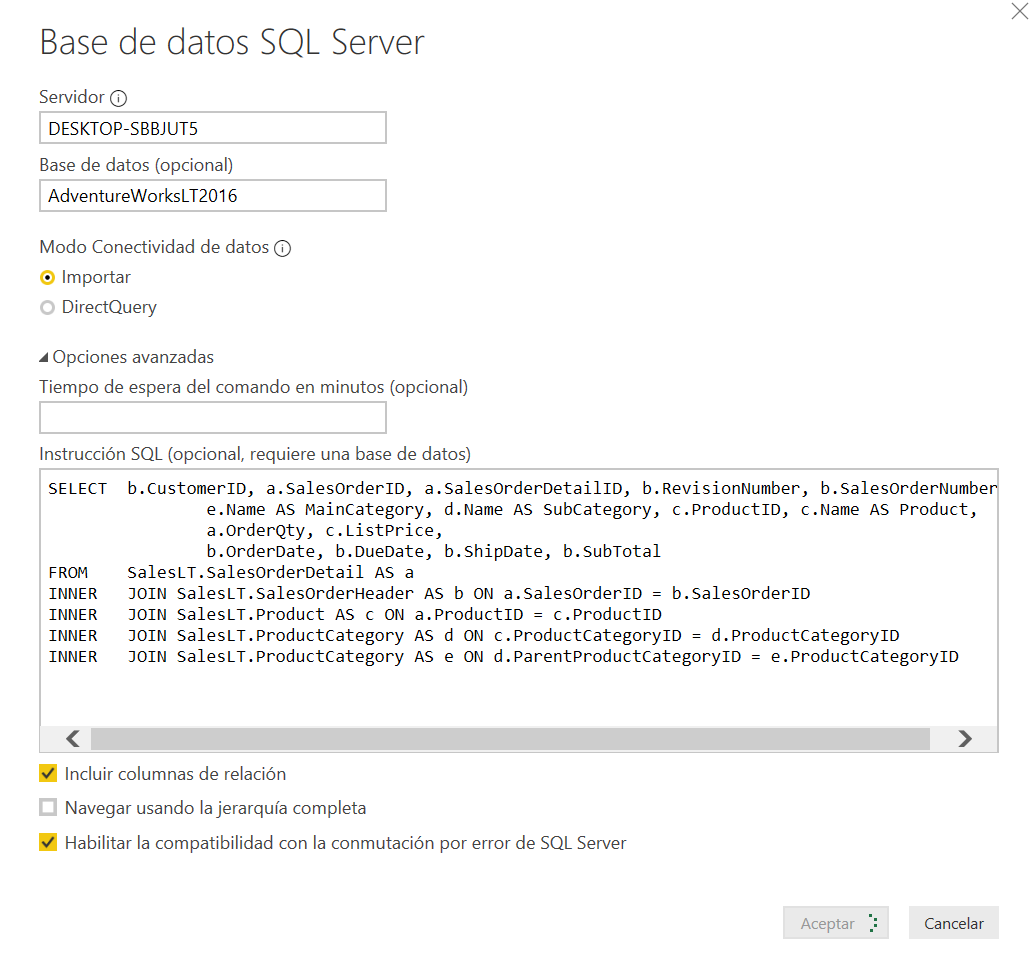
\includegraphics[scale=0.55]{./Imagenes/9.png}
\end{center}

\item Guardarlo como AdventureWorksLT Sales.pbix De manera que   lo que nos debe salir al hacer click en Datos sea:

\begin{center}
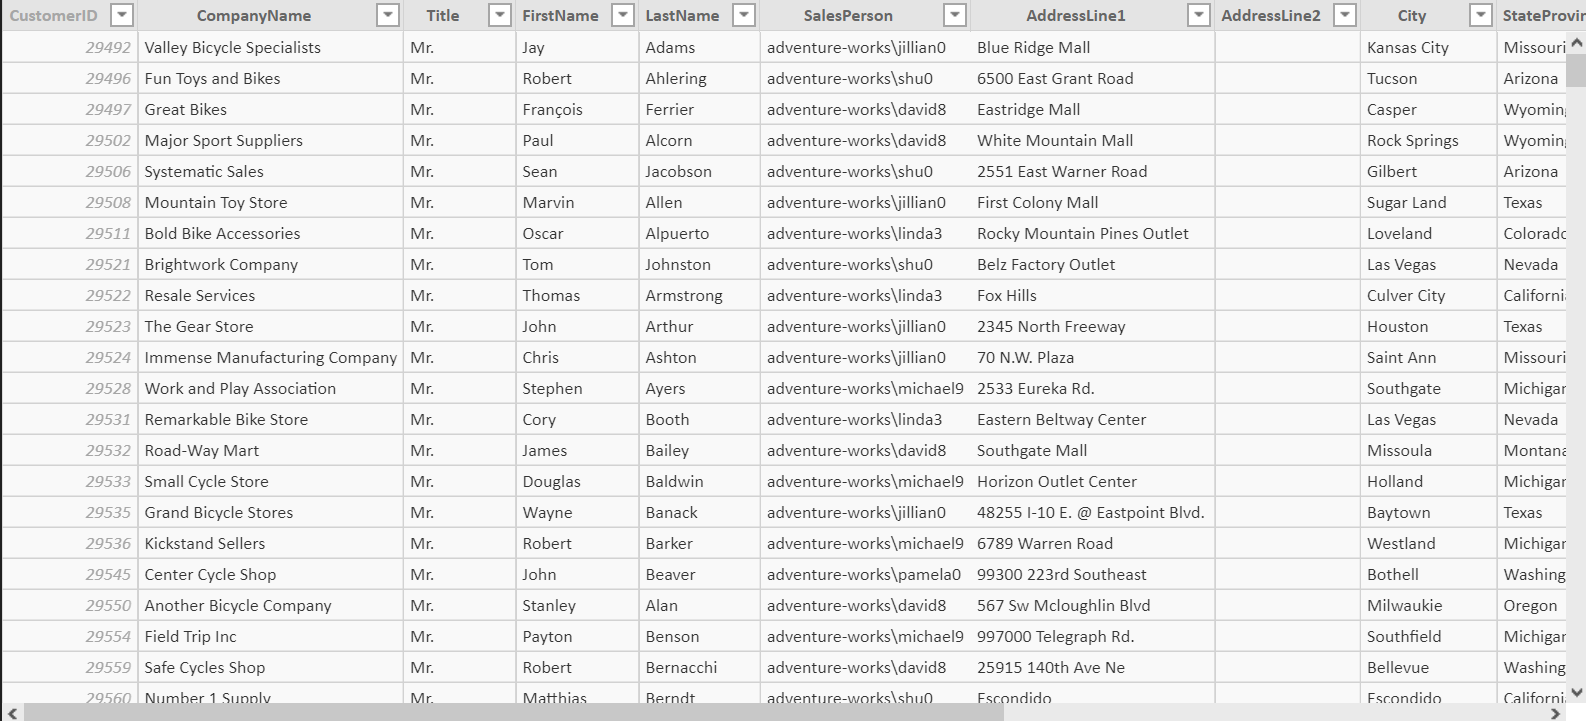
\includegraphics[scale=0.55]{./Imagenes/tarea1_final.png}
\end{center}
\begin{center}
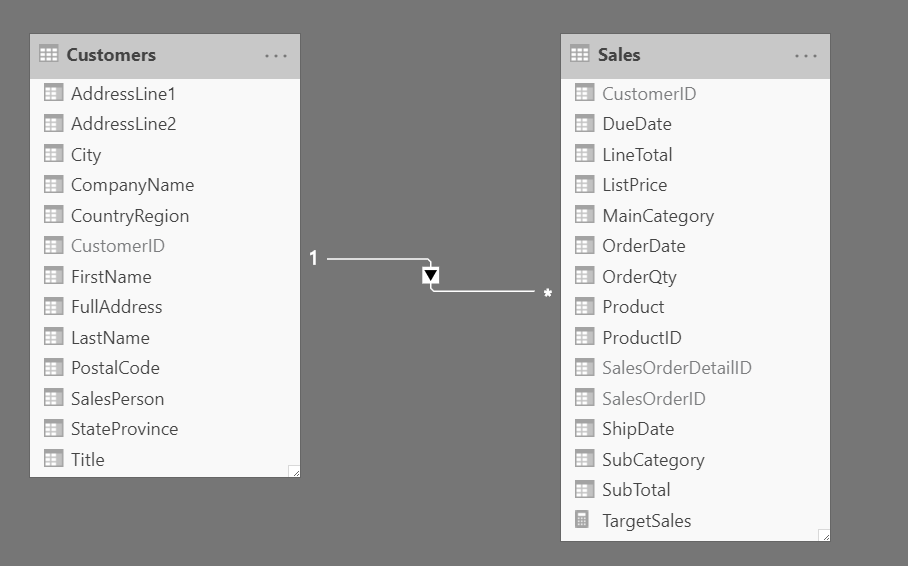
\includegraphics[scale=0.55]{./Imagenes/tarea1_final_2.png}
\end{center}

\end{enumerate}



\item Tarea 2 : Formar Datos


\begin{enumerate}
\item Renombrar ambas consultas creadas de la Tarea 1 y renombrar el primero Query como Customers .De la misma manera con el Query2 como Sales

\begin{center}
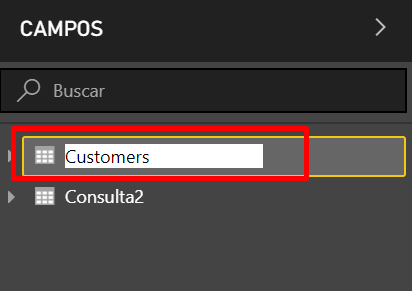
\includegraphics[scale=0.55]{./Imagenes/12.png}
\end{center}

\begin{center}
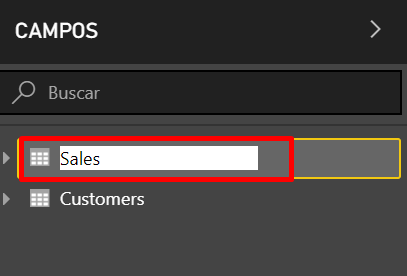
\includegraphics[scale=0.55]{./Imagenes/13.png}
\end{center}

\item De la tabla Customers eliminar las filas NameStyle , SalesPerson . Tambien en las filas AddressLine1, City , StateProvince ,ContryRegion y PostalCode hacer click en Modelado  y en Categoria de datos : Sin clasificar 	

\begin{center}
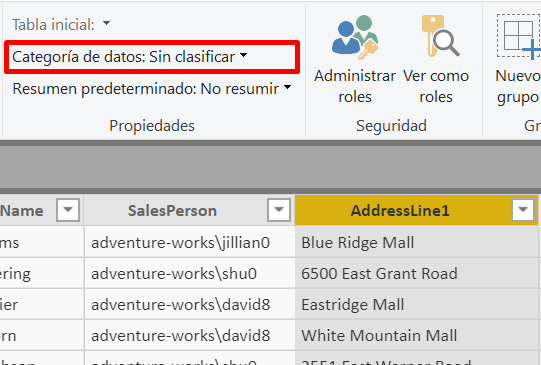
\includegraphics[scale=0.55]{./Imagenes/20.png}
\end{center}

\begin{center}
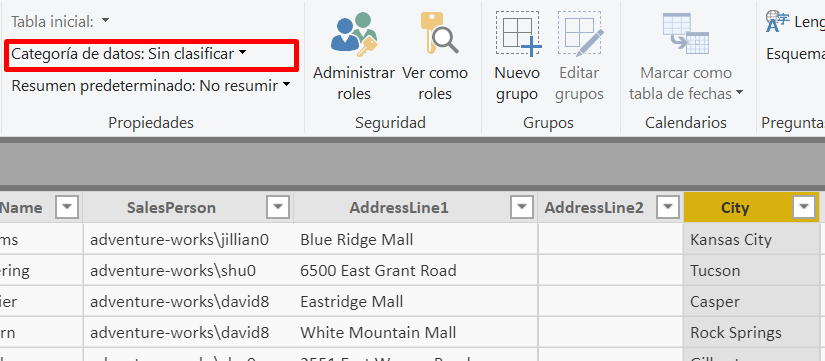
\includegraphics[scale=0.55]{./Imagenes/21.png}
\end{center}

\begin{center}
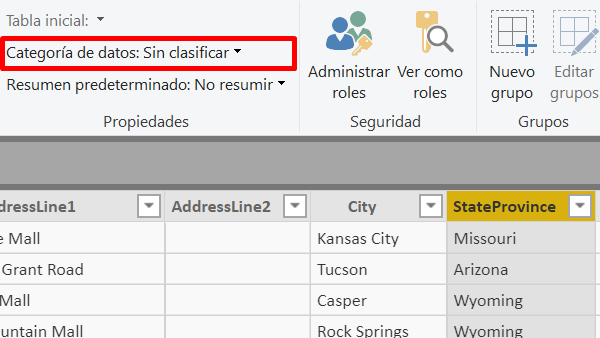
\includegraphics[scale=0.55]{./Imagenes/22.png}
\end{center}

\begin{center}
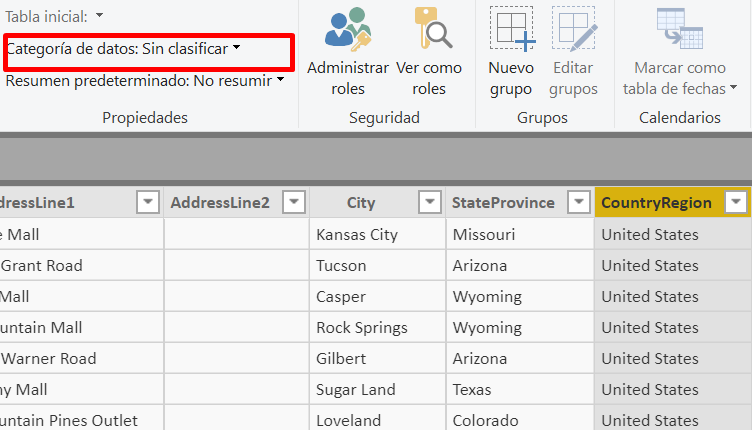
\includegraphics[scale=0.55]{./Imagenes/23.png}
\end{center}

\begin{center}
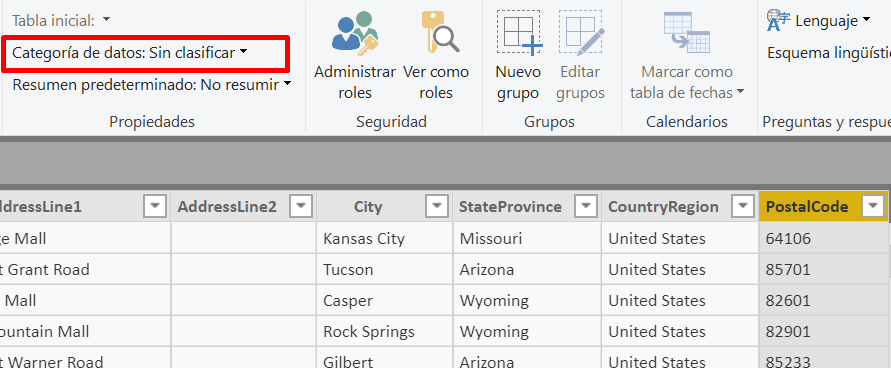
\includegraphics[scale=0.55]{./Imagenes/24.png}
\end{center}

\item Agregar una nueva Columna en la parte de Calculos en nueva columna y copiar la siguiente formula

\begin{center}
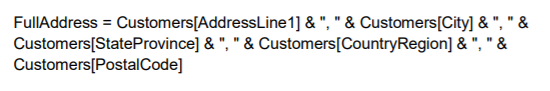
\includegraphics[scale=1]{./Imagenes/tarea2_formula.png}
\end{center}

\item En la tabla Sales , eliminar as filas RevisionNumer y SalesOrderNumer. Tambien ocultar en la vista de informes las columnas CustomerID, SalesOrderID, SalesOrderDetailID
\begin{center}
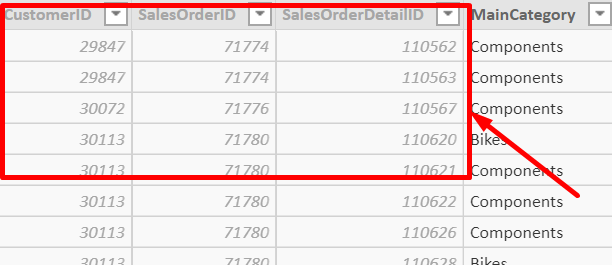
\includegraphics[scale=0.55]{./Imagenes/29.png}
\end{center}

\item Agregar una nueva Columna en la parte de Calculos en nueva columna y copiar la siguiente formula

\begin{center}
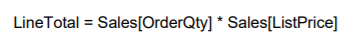
\includegraphics[scale=1]{./Imagenes/tarea2_formula2.png}
\end{center}

\item Hacer click en LineTotal	 y en el menu de herrameintas superior  en Modelado en cuadro de Formato , hacer click en Formato:General y en Moneda colocar English (United States) y Guardar lo avanzado.

\begin{center}
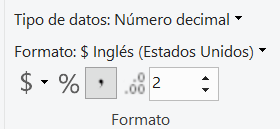
\includegraphics[scale=1]{./Imagenes/31.png}
\end{center}


\end{enumerate}



\item Tarea 3 : Combinar Datos


\begin{enumerate}
\item Abrir el archivo State.xlsx y hacer Ctrl+ C a la tabla . Seguidamente Abrir PowerBI y en el cuadro de Datos externos hacer click en Especificar Datos y hacer Ctrl+ V 

\begin{center}
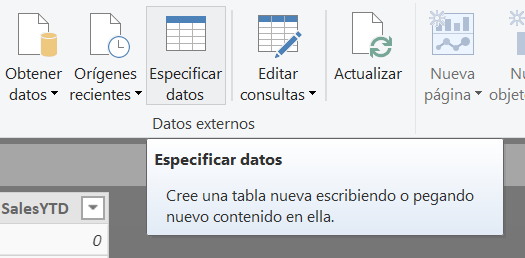
\includegraphics[scale=0.55]{./Imagenes/tarea3_creartabla.png}
\end{center}

\begin{center}
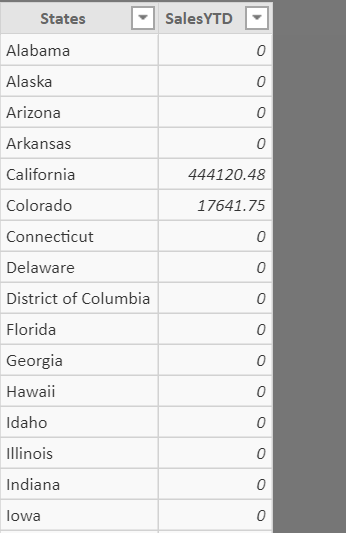
\includegraphics[scale=0.55]{./Imagenes/tarea3_tabla.png}
\end{center}

\item Renombrar la tabla creada a Sales by State.

\begin{center}
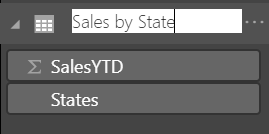
\includegraphics[scale=0.55]{./Imagenes/tarea3_cambiarnombre.png}
\end{center}

\item Despues abrir en PowerBI en Obtener Datos y en Web , poniendo la siguiente URL:

\begin{center}
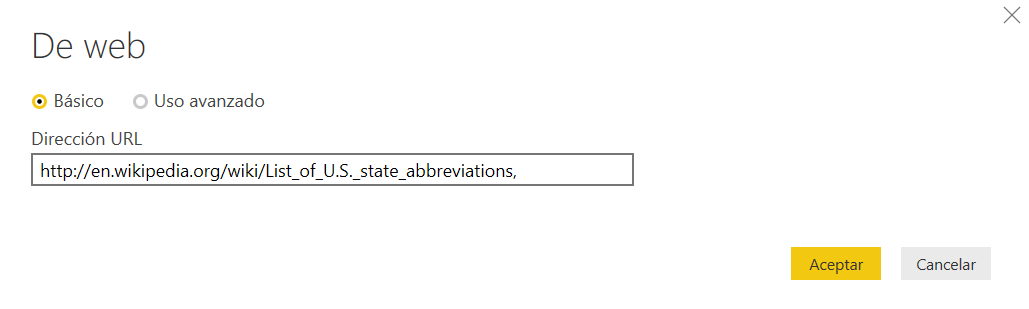
\includegraphics[scale=0.55]{./Imagenes/tarea3_URL.png}
\end{center} 

\item Seguidamente escoger la tabla Codes and abbreviations for U.S. states, territories and other regions y cargar datos . Hacer click en Editar Consultas . En la ventana emergente hacer click en Reducir Filas despues en Quitar Filas y en Quitar filas inferiores , especificando las 26 ultimas filas en la ventana emergente.

\begin{center}
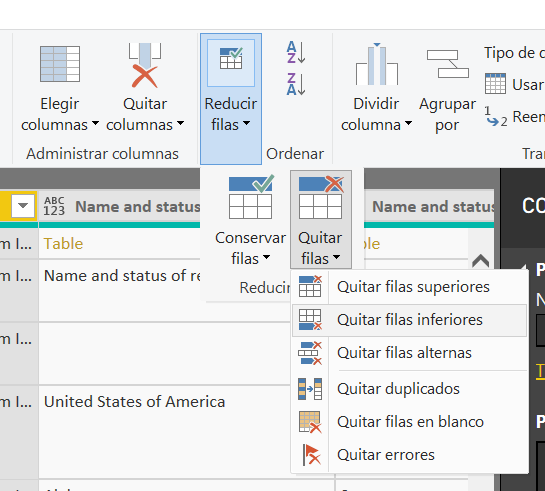
\includegraphics[scale=0.55]{./Imagenes/tarea3_removerows.png}
\end{center}

\begin{center}
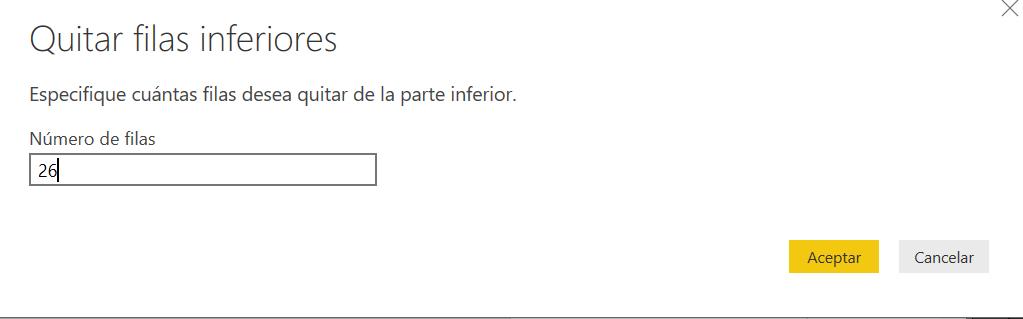
\includegraphics[scale=0.55]{./Imagenes/tarea3_26rows.png}
\end{center}


\item 

\begin{center}
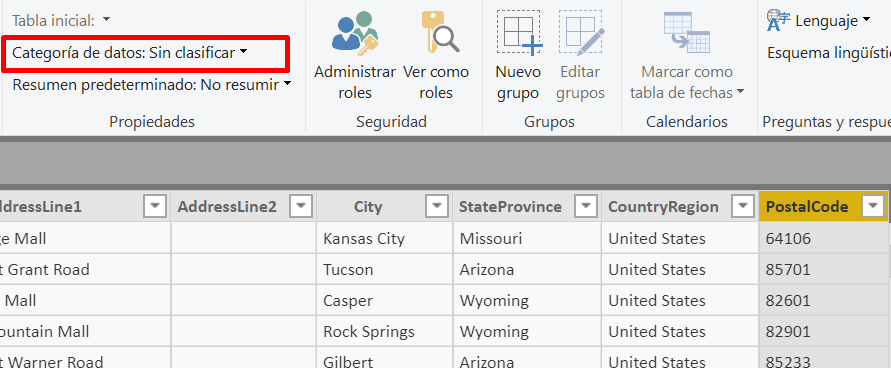
\includegraphics[scale=0.55]{./Imagenes/24.png}
\end{center}

\item Agregar una nueva Columna en la parte de Calculos en nueva columna y copiar la siguiente formula

\begin{center}
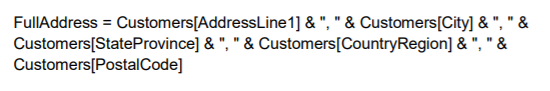
\includegraphics[scale=1]{./Imagenes/tarea2_formula.png}
\end{center}

\item En la tabla Sales , eliminar as filas RevisionNumer y SalesOrderNumer. Tambien ocultar en la vista de informes las columnas CustomerID, SalesOrderID, SalesOrderDetailID
\begin{center}
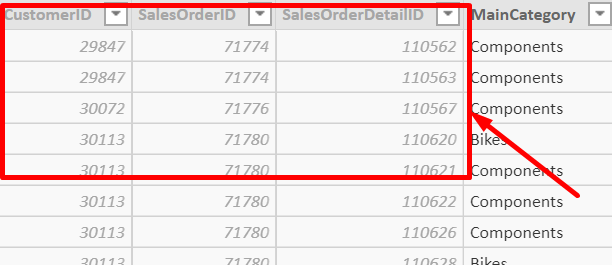
\includegraphics[scale=0.55]{./Imagenes/29.png}
\end{center}

\item Agregar una nueva Columna en la parte de Calculos en nueva columna y copiar la siguiente formula

\begin{center}
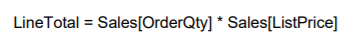
\includegraphics[scale=1]{./Imagenes/tarea2_formula2.png}
\end{center}

\item Hacer click en LineTotal	 y en el menu de herrameintas superior  en Modelado en cuadro de Formato , hacer click en Formato:General y en Moneda colocar English (United States) y Guardar lo avanzado.

\begin{center}
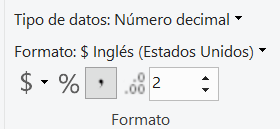
\includegraphics[scale=1]{./Imagenes/31.png}
\end{center}

\item Seleccionar las columnas de ASNI2 , AP, GPO, Header, Name and status of region2, Other abbreviations , USCG y USPS y eliminarlas. Seguidamente en el cuadro de Consulta en Propiedades , en Nombre poner States with Code y Aceptar.
\item Despues  en el cuadro de Transformar de menu , hacer click en Usar la primera fila como encabezado de tal manera que Renombrando United States of America por State Name , US USA 840 por State Code Long y US por State Code Short y Aceptar. Debe aparecer de esta manera la tabla generada:
\begin{center}
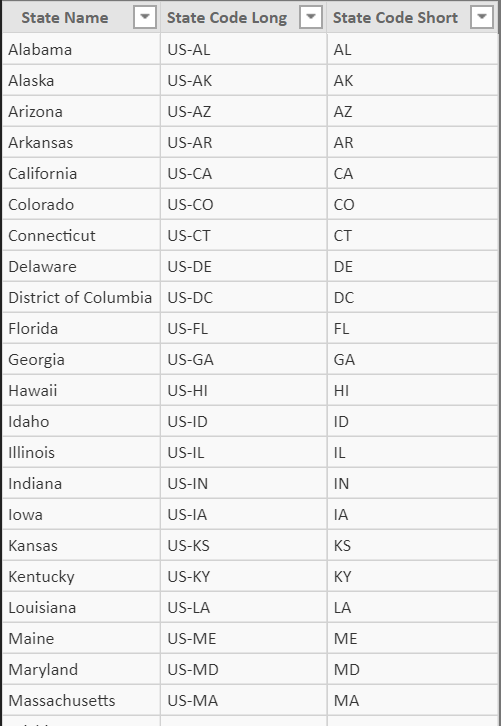
\includegraphics[scale=1]{./Imagenes/tarea3_renombrartablas.png}
\end{center}

\item En el cuadro  Combinar , hacer click en Combinar Consultas . En la ventana emergente de la tabla Sales by State seleccionar la columna States y en la iguiente tabla escoger States with Code y seleccionar la columna StateName y aceptar . Renombrar el nombre de la fila  nueva a State Code y expandir , seleccionando solo State Code Short y Aceptar.

\begin{center}
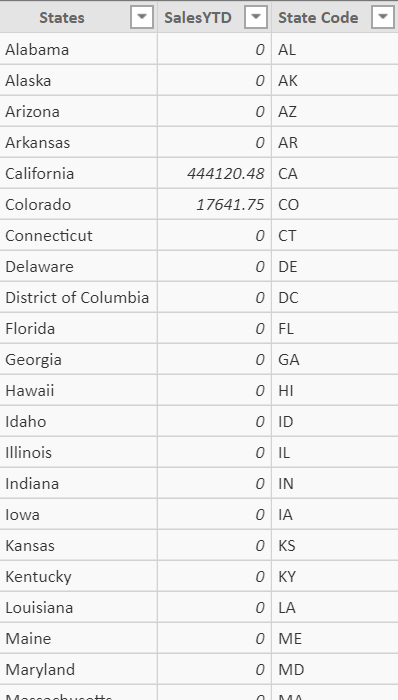
\includegraphics[scale=1]{./Imagenes/tarea3_tablacombinada.png}
\end{center}

\item Como ultimo paso Ocultar de ls vista de informes la tabla States with Code.
\begin{center}
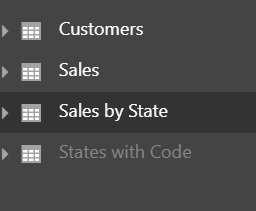
\includegraphics[scale=1]{./Imagenes/tarea3_ocultartabla.png}
\end{center}
\end{enumerate}


EJERCICIO 2 : Construyendo Reportes en PowerBI

\begin{enumerate}
\item Tarea 1 : Crear un Grafico

\begin{center}
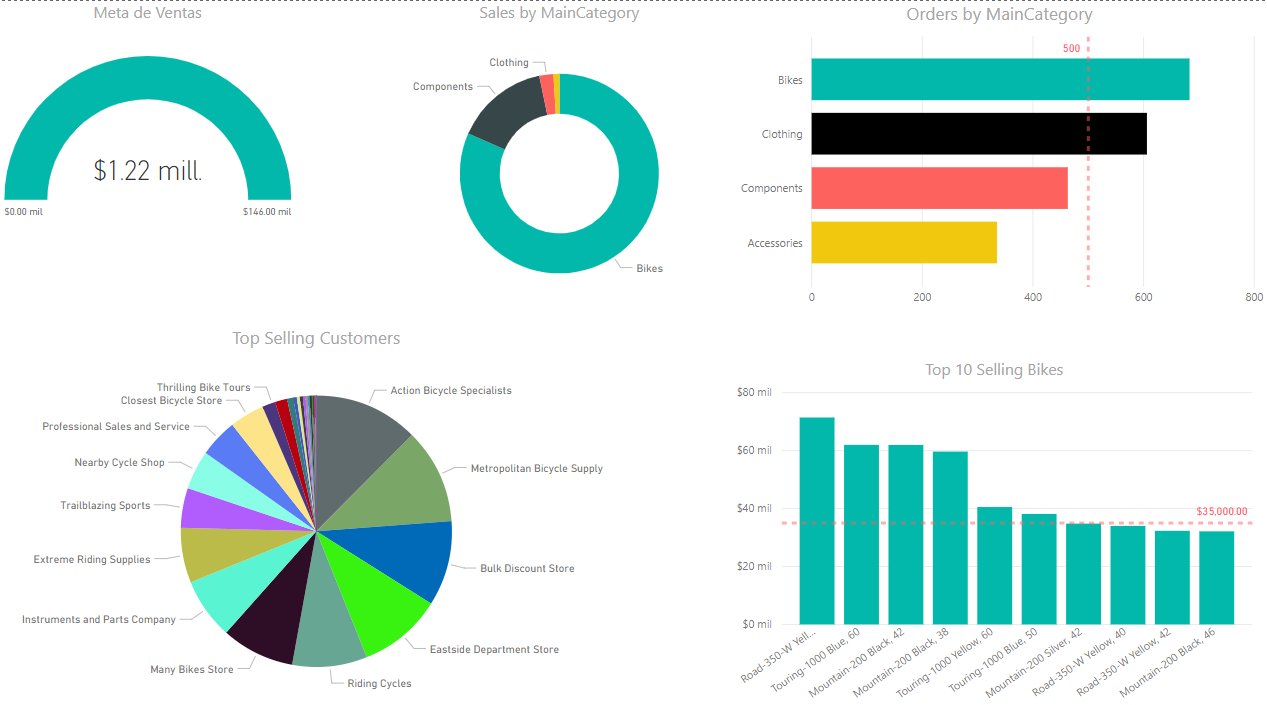
\includegraphics[scale=0.66]{./Imagenes/ejer2_tarea1.png}
\end{center}

\item Tarea 2: Crear una Visualizaci\'on de Mapa a Map Visualization

\begin{center}
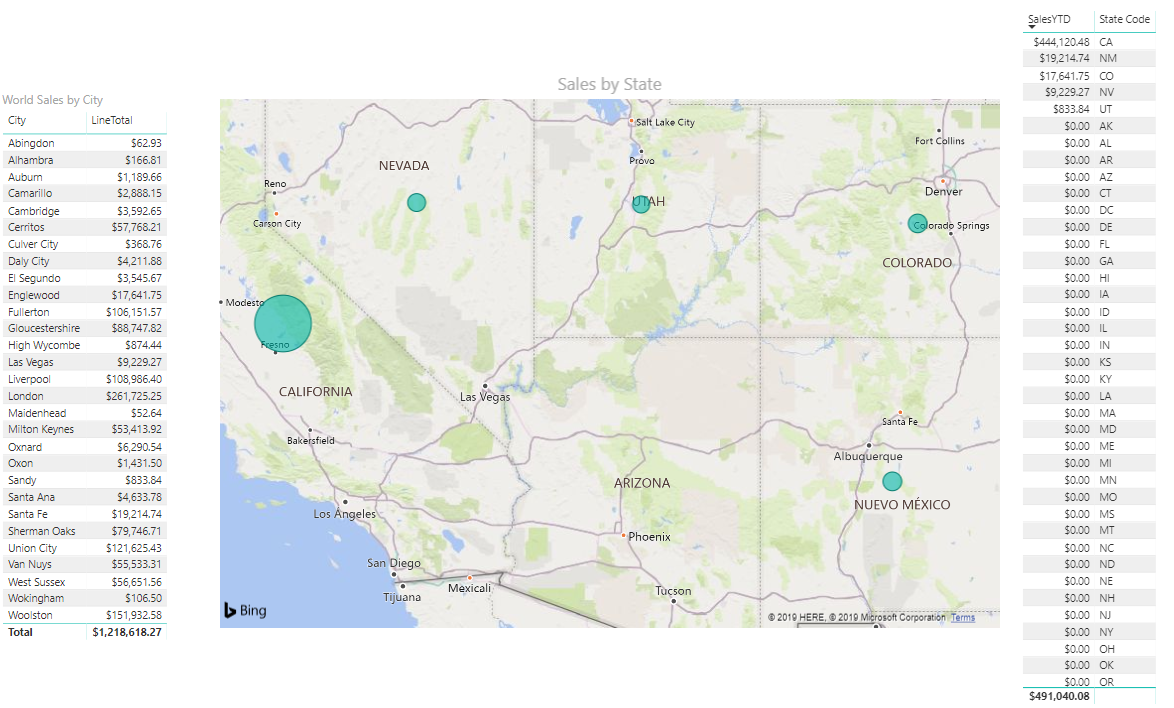
\includegraphics[scale=0.70]{./Imagenes/ejer2_tarea2.png}
\end{center}

\end{enumerate}


EJERCICIO 3 : Creando un Panel en PowerBI
\begin{enumerate}

\item Tarea 1 :Publicar todo lo avanzado hasta ahora . Asegurar de iniciar correctamente las sesiones solicitadas.

\begin{center}
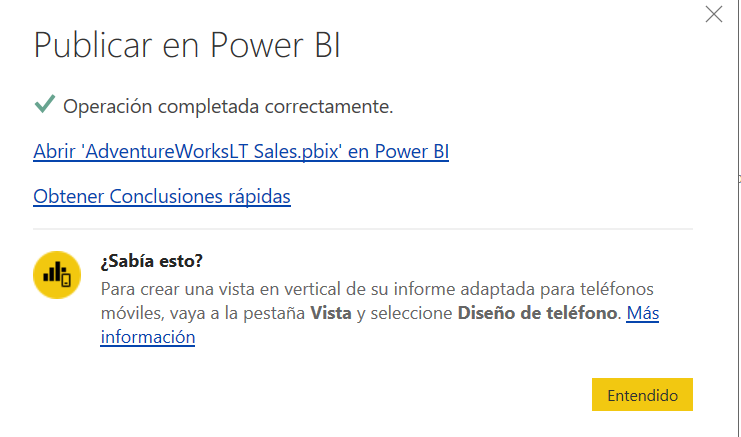
\includegraphics[scale=0.66]{./Imagenes/ejer3_publicar.png}
\end{center}

\item Tarea 2: Crear una Visualizaci\'on de Mapa a Map Visualization : En Informes, haga clic en Ventas de AdventureWorksLT y seguidamente por cada grafico creado anclar y agregar el titulo igual que el creado y un subtitulo.

\begin{center}
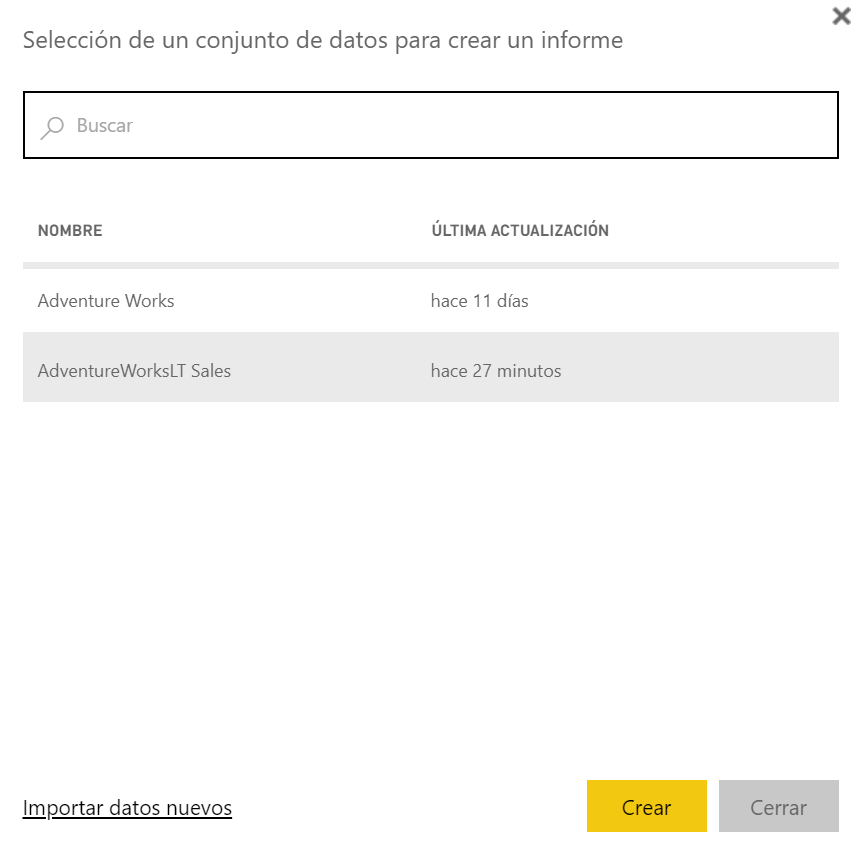
\includegraphics[scale=0.70]{./Imagenes/ejer3_clickBD.png}
\end{center}

\begin{center}
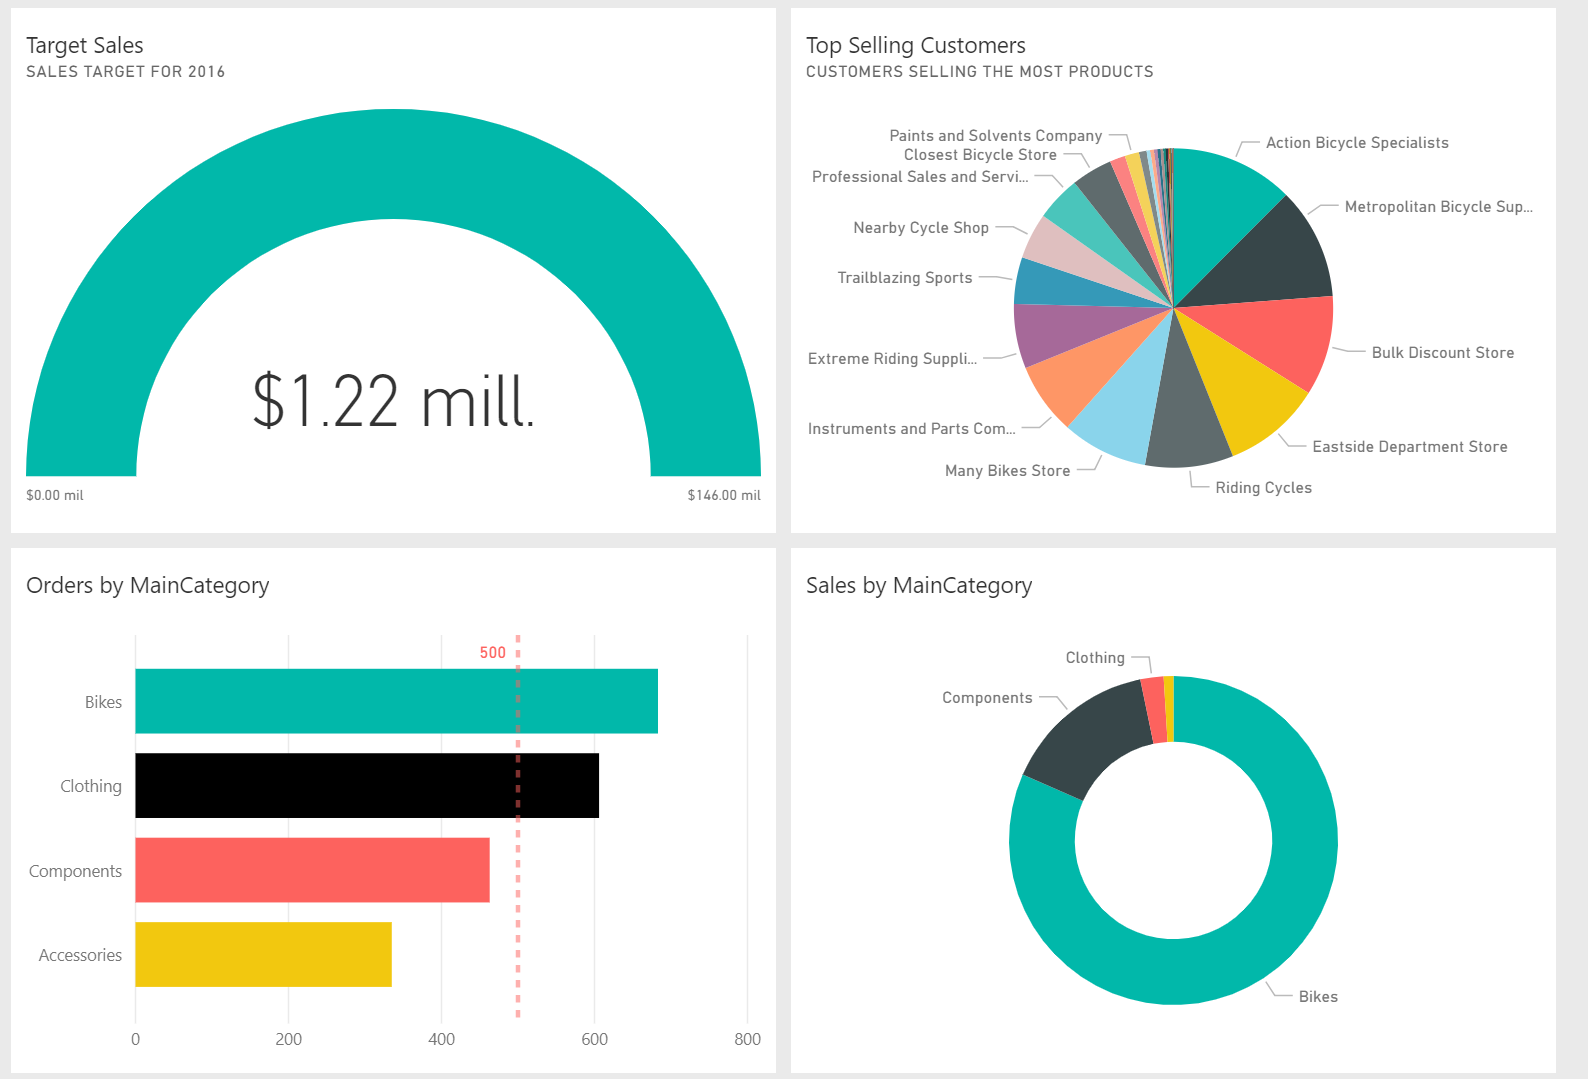
\includegraphics[scale=0.60]{./Imagenes/ejer3_panel1.png}
\end{center}
\begin{center}
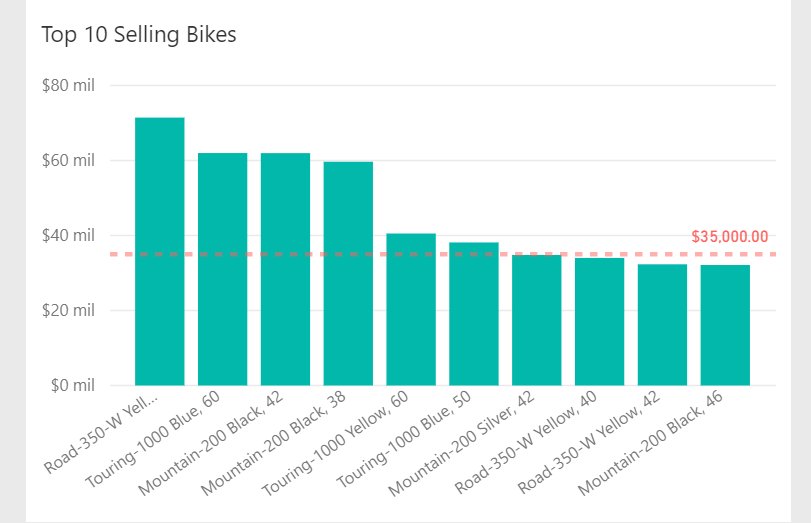
\includegraphics[scale=0.55]{./Imagenes/ejer3_panel2.png}
\end{center}

Link Power BI : https://app.powerbi.com/groups/me/reports/2373da12-e413-436d-bf33-79535dc55b71/ReportSection

\end{enumerate}

\end{itemize}







 	 	


\end{document}
